\documentclass[a4paper,11pt,fleqn]{article}%fleqn pour aligner les equations à gauche
\usepackage{../../Styles/Cours}

\newcommand{\chnum}{Chapitre 16}
\newcommand{\chtitle}{La réfraction}
\newcommand{\dtype}{TP}

\begin{document}
\maketitle
\section{Mise en situation}
\begin{minipage}{.8\linewidth}
	Lorsque la lumière passe d'un milieu à un autre, deux phénomènes se mettent en place :
	\begin{itemize}
		\item Une partie de la lumière est reflétée par la surface, agissant comme un miroir
		\item Une autre partie de la lumière est réfractée : sa direction de propagation change. c'est ce phénomène qui est à l'origine des déformations apparentes que l'on constate lorsque l'on regarde un objet dans l'eau.
	\end{itemize}
\end{minipage}
\begin{minipage}{.15\linewidth}
	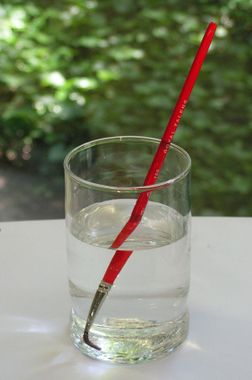
\includegraphics[width=\linewidth]{Ressources/Pinceau.jpeg.jpg}
\end{minipage}

\section{Le phénomène de réfraction}
Le phénomène de réfraction vient du fait que la lumière se déplace à une vitesse diféfrente selon le milieu dans lequel il se propage : dans le vide ou dans l'air, la lumière a une vitesse maximale (notée $c=\SI{3E8}{\meter\per\second}$), dans d'autres milieux on utilise l'\textit{indice de  réfraction} (nopté : $n_{milieu}$) définit comme le rapport entre la vitesse de la lumière dans le vide et dans une autre milieu (notée : $v_{milieu}$) : 
$$n_{milieu}=\dfrac{c}{v_{milieu}} $$
$n$ n'a pas d'unité et est toujours >1 car il n'est pas possible de dépasser la valeur de $c$.\\
Une valeur de $n$ grande indique que la limère y est ralentie de manière importante et donnera une réfraction plus grande.

\section{Schématiser la situation :}
\begin{figure}[h!]
	\begin{minipage}{.5\linewidth}
	\begin{tikzpicture}[scale=.75,transform shape]
	\fill[gray!30] (-6,0)--(6,0)--(6,-5)--(-6,-5)--cycle;

	\draw[thick] (-6,0)--(6,0);
	\draw[thick,dashed] (0,-5)--(0,5);
	\draw[thick,red,-Stealth] (-5,5) to (-2.5,2.5);
	\draw[thick,red] (-2.5,2.5) -- (0,0);

	\draw[thick,blue,-Stealth] (0,0) to (1.5,-3);
	\draw[thick,blue] (1.5,-3) -- (2.5,-5);

	\draw[thick,green!60!black,-Stealth] (0,0) to (2.5,2.5);
	\draw[thick,green!60!black] (2.5,2.5) -- (5,5);

	\node[above] (m1) at (-5,0){Milieu 1};
	\node[below] (m2) at (-5,0){Milieu 2};
	\end{tikzpicture}
\end{minipage}
\begin{minipage}{.5\linewidth}
	\textbf{Les lois de Snell-Descartes}\\
	On appelle :
le \textbf{dioptre}, l'interface entre les deux milieux transparents ;
le \textbf{rayon incident}, le rayon lumineux arrivant au dioptre ;
La \textbf{normale}, la droite perpendiculaire au dioptre, passant par le point d'incidence
l’\textbf{angle d’incidence}, noté $i_1$ l’angle formé par le rayon incident et la normale du dioptre ;
l’\textbf{angle de réfraction}, noté $i_2$ , est l’angle formé par le rayon réfracté et la normale du dioptre ;
l’\textbf{angle de réflexion}, noté $r$ , est l’angle formé par le rayon réfléchi et la normale.\\
%\hlinefill
Les lois de Snell-Descartes ont été établies indépendamment par Willebrord Snell et René Descartes au XVIIe siècle.
\begin{itemize}
	\item \underline{1ère loi de Snell-Descartes} : le rayon incident, le rayon réfracté, le rayon réfléchi et la normale sont dans le même plan.
	\item \underline{2ème loi de Snell-Descartes} :
	\begin{itemize}
		\item pour la réfraction : $n_1 \cdot sin(i_1)=n_2 \cdot sin (i_2)$
		\item pour la réflexion : $i_1=r$
	\end{itemize} 
\end{itemize}
\end{minipage}
\end{figure}

\newpage
\section{Activité Expérimentale :}
Une lanterne émet un faisceau rectiligne dont le trajet peut être observé sur un disque gradué en degrés.
\begin{itemize}
	\item Allumer la lanterne et aligner le faisceau pour qu’il passe par la graduation zéro et le centre du disque.
    \item Poser le demi-cylindre en plexiglas au centre du disque gradué.
    \item On peut repérer à l’aide des graduations les valeurs des angles $i_1$ et $i_2$.
    \item On peut déplacer le disque et le demi-cylindre de manière à faire varier la valeur de l’angle d’incidence $i_1$.
   \end{itemize}
\begin{enumerate}
	\item Régler le disque pour obtenir $i_1$ = 40°. Noter la valeur que prend l'angle de réfraction $i_2$. Faire valider cette valeur par le professeur.\vspace*{1cm}
	\item Représenter la situation précédente à l'aide d'un schéma légendé.\vspace*{3cm}
	\item Faire varier $i_1$ entre 0 et 70° et mesurer chaque valeur de $i_2$ pour compléter le tableau suivant :\\
	\begin{tabular}{|>{\centering}m{.08\textwidth}|>{\centering}m{.08\textwidth}|>{\centering}m{.08\textwidth}|>{\centering}m{.08\textwidth}|>{\centering}m{.08\textwidth}|>{\centering}m{.08\textwidth}|>{\centering}m{.08\textwidth}|>{\centering}m{.08\textwidth}|>{\centering\arraybackslash}m{.08\textwidth}|}
	\hline
	$i_1$ (en °) & 0 & 10 & 20 & 30 & 40 & 50 & 60 & 70\\
	\hline
	$i_2$ (en °) &  &  &  &  &  &  &  & \rule[1cm]{0cm}{0cm}\\
	\hline
	\end{tabular}
	\item Calculer les valeurs de $sin(i_1)$ et $sin(i_2)$ pour compléter le tableau suivant :\\
	\begin{tabular}{|>{\centering}m{.08\textwidth}|>{\centering}m{.08\textwidth}|>{\centering}m{.08\textwidth}|>{\centering}m{.08\textwidth}|>{\centering}m{.08\textwidth}|>{\centering}m{.08\textwidth}|>{\centering}m{.08\textwidth}|>{\centering}m{.08\textwidth}|>{\centering\arraybackslash}m{.08\textwidth}|}
	\hline
	$sin(i_1)$ &  &  &  &  &  &  &  & \rule[1cm]{0cm}{0cm}\\
	\hline
	$sin(i_2)$ &  &  &  &  &  &  &  & \rule[1cm]{0cm}{0cm}\\
	\hline
	\end{tabular}
	\item À partir des lois de Snell-Descartes, déterminer ce que représente le rapport $\dfrac{sin(i_1)}{sin(i_2)}$.\vspace*{2cm}
	\item Compléter le tableau suivant :\\
	\begin{tabular}{|>{\centering}m{.08\textwidth}|>{\centering}m{.08\textwidth}|>{\centering}m{.08\textwidth}|>{\centering}m{.08\textwidth}|>{\centering}m{.08\textwidth}|>{\centering}m{.08\textwidth}|>{\centering}m{.08\textwidth}|>{\centering}m{.08\textwidth}|>{\centering\arraybackslash}m{.08\textwidth}|}
	\hline
	$\dfrac{sin(i_1)}{sin(i_2)}$ &  &  &  &  &  &  &  & \rule[1cm]{0cm}{0cm}\\
	\hline
	\end{tabular}
	\item Calculer la moyenne des valeurs obtenues pour la question 6. et exprumer une valeur moyenne de $n_2$.
\end{enumerate}
\end{document}
